\subsection{VGGT / Depth-Guided Densification}
\label{sec:depth_densify}

The Visual Hull provides a stable coarse geometric prior, but silhouette constraints alone cannot fully recover concave regions and fine structures. We therefore densify the Visual Hull point cloud with \textbf{VGGT-Depth}: starting from a pre-trained VGGT backbone~\cite{ref30}, we train a depth prior adaptation branch with cross-attention over multi-view tokens and a lightweight fusion head to predict per-view depth maps and confidence estimates under a shared geometric context. As illustrated in Fig.~\ref{fig:vggt_depth}, these adapted multi-view depth priors are used to identify reliable observations, supplement missing geometry, and assist Gaussian attribute initialization. Our remaining design then focuses on reliable depth selection, 3D point supplementation and fusion, and using these cues for Gaussian initialization.

% Placeholder — replace path when the figure is ready
% \begin{figure}[ht]
% \centering
% 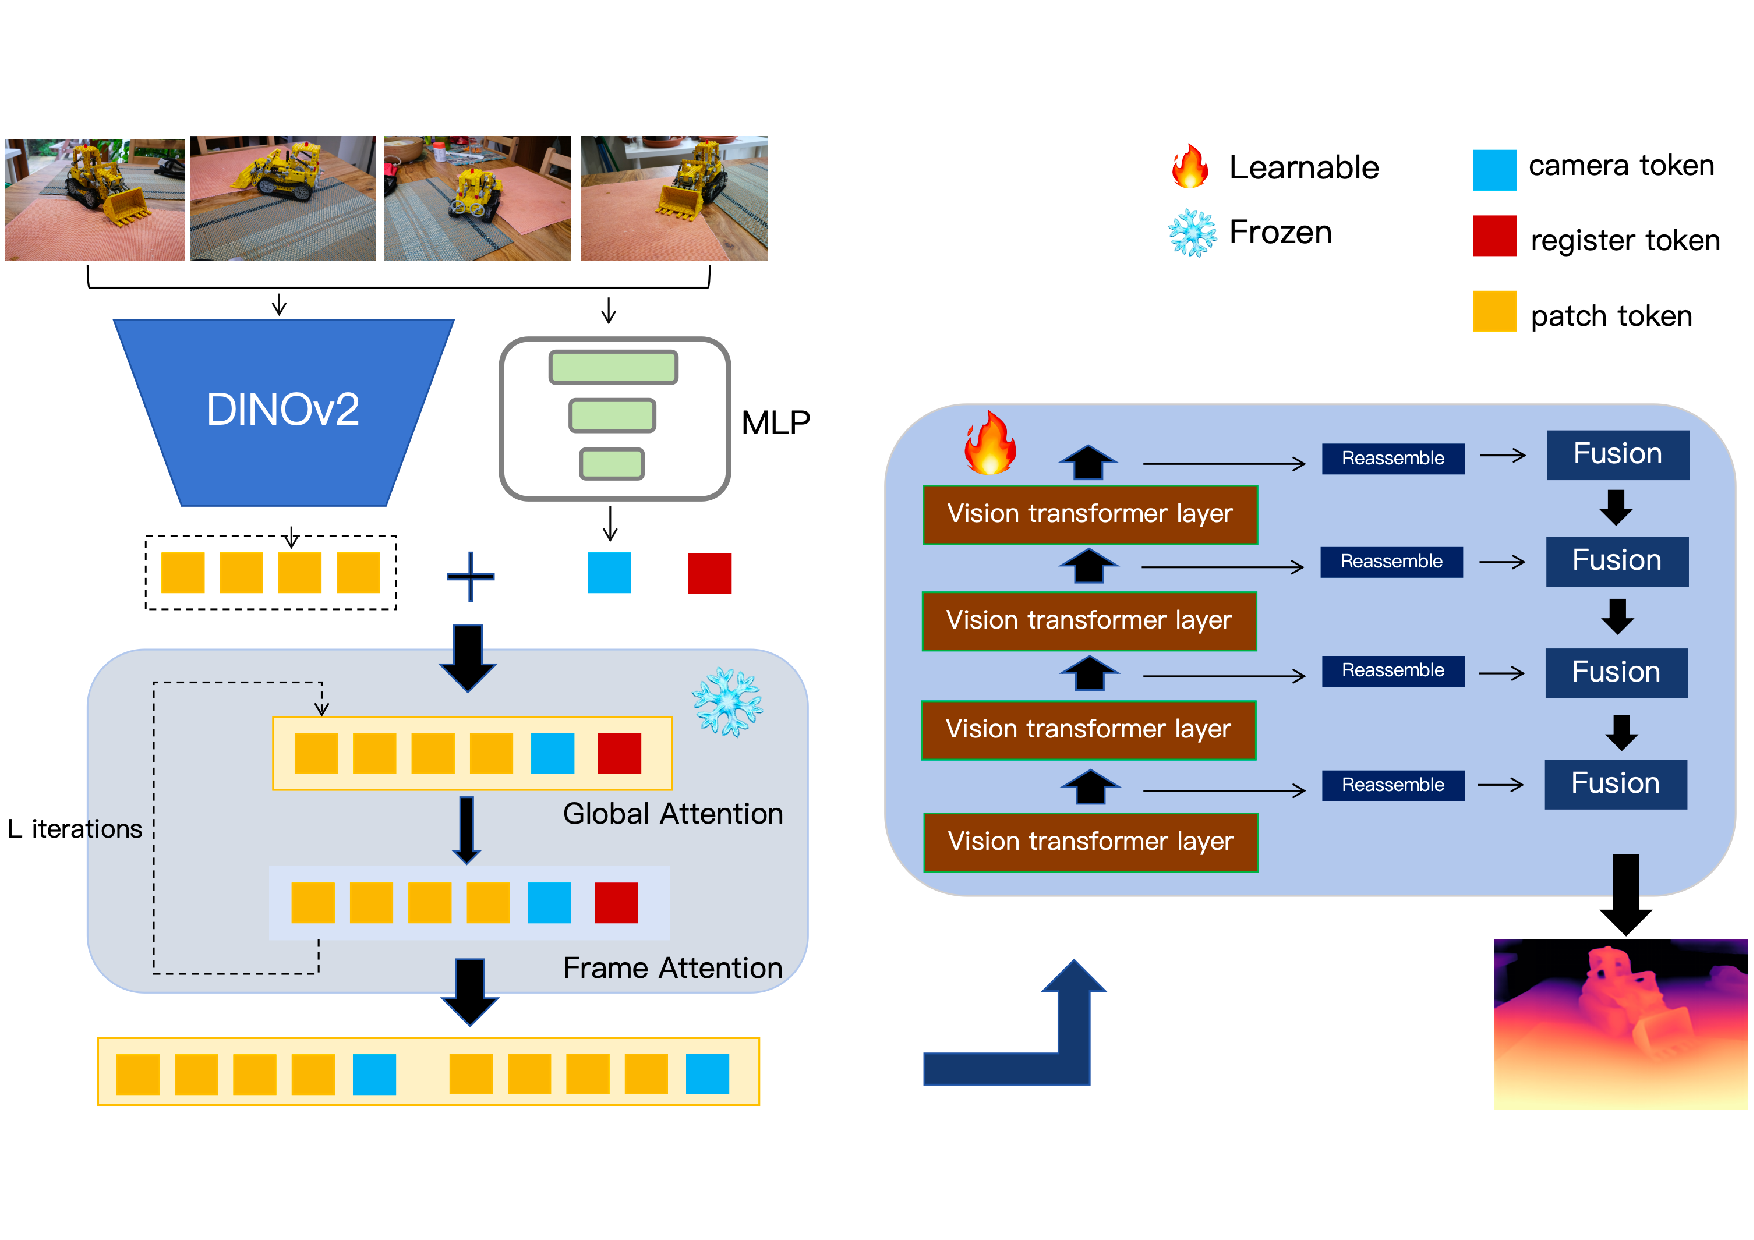
\includegraphics[width=\textwidth]{figures/vggt_depth.pdf}
% \caption{VGGT-Depth prior used for depth-guided point cloud densification.}
% \label{fig:vggt_depth}
% \end{figure}

We use the diagonal length $L$ of the Visual Hull AABB as the scene-scale reference. Before point supplementation, the predicted depth maps are screened at both the view and ray levels. For each view, the masked depth MAE against the dataset ground-truth depth is normalized by the 95th percentile over the validation views to obtain a quality score $q_v$. Views with $q_v<0.4$ are discarded. If fewer than $0.8N$ views remain, depth densification is skipped and the original Visual Hull point cloud is retained. For the selected views, reliable regions are further determined using the VGGT-Depth prediction, its confidence, and depth consistency. We use a depth-adaptive tolerance
\begin{equation}
\label{eq:delta_d}
\Delta(d)=\alpha d+\beta,\qquad
\alpha=0.01,\quad \beta=0.002L,
\end{equation}
and reject low-confidence or depth-inconsistent observations before back-projection.

Point supplementation is performed only along reliable rays. For each point to be supplemented, the top $K=3$ reliable views are selected, and candidate points are sampled around the predicted depth and back-projected into 3D. The supplementary points are merged with the Visual Hull point cloud through two-stage voxel fusion and deduplication, using voxel sizes of $0.01L$ and $0.004L$ for coarse merging and local uniformization, respectively. The resulting densified point cloud provides the geometric input for Gaussian initialization.

Each densified point directly initializes a Gaussian center, while its scale is estimated from the average distance to its $k=8$ nearest neighbors. Multi-view colors are fused using depth-consistency and VGGT confidence weights for appearance initialization. Opacity is initialized from the corresponding cross-view consistency scores and clipped to $[0.2,0.8]$. This process converts the coarse Visual Hull prior into a more complete Gaussian initialization. Sparse-view optimization can still produce uneven supervision across Gaussian primitives with different visibility. We address this issue in the next stage using DVR (Sec.~\ref{sec:dvr}).
